\section{Vérification des propriétés pour les opérateurs}
Rappel :
Définition et propriétés d'un opérateur d'agrégation : $Agg: \underset{n\in \mathds{N}}{\cup}[0,1]^n\to [0,1]$
\begin{itemize}
    \item identité si $n=1 : Agg(u)=u$
    \item conditions aux limites : $Agg(0,\dots,0)=0$ et $Agg(1,\dots,1)=1$
    \item monotonie croissante : $Agg(u_1,\dots,u,\dots,u_n)\leq Agg(u_1,\dots,v,\dots,u_n)$ si $u \leq v$
\end{itemize}

\subsection{Opérateur géométrique}
Soit $\varepsilon>0$
    \begin{equation}
            agg_{geo}(s_0,s_1,\dots,s_{n-1}) =\exp\left( \frac{1}{N} \sum_{i<n} \log(\max(s_i,\varepsilon ))\right) 
    \end{equation}

\paragraph{Identité}
$$agg_{geo}(u) = \exp(\log(\max(u,\varepsilon))) = \max(u,\varepsilon)$$
Si $u<\varepsilon$, $agg_{geo}(u)=\varepsilon \neq u$. La propriété d'identité n'est pas respectée.

\paragraph{Conditions aux limites}
$$agg_{geo}(0,\dots,0) =\exp\left( \frac{1}{N} \sum_{i<n} \log(\varepsilon)\right) =  \varepsilon\neq 0$$

$$agg_{geo}(1,\dots,1) =\exp\left( \frac{1}{N} \sum_{i<n} \log(1)\right) =  1$$
Pour la limite en zéro la condition n'est pas respectée.

Les propriétés d'identité et de conditions aux limites ne sont plus respecté après l'ajout de $\varepsilon$ (contrairement à la moyenne géométrique classique). Cependant, nous considérons ces propriétés moins déterminante pour notre application par rapport à l'avantage d'ajouter $\varepsilon$  comme discuté dans la section \ref{op_geo}.

\paragraph{Monotonie croissante}
Soit $u \leq v$, $Agg(u_1,\dots,u,\dots,u_n)$ ne diffère de $ Agg(u_1,\dots,v,\dots,u_n)$ que par un seul terme de la somme.
On veut montrer que $\log(\max(u,\varepsilon))\leq \log(\max(v,\varepsilon))$, hors $\max(u,\varepsilon) \leq \max(v,\varepsilon)$ et donc par croissance du log, on obtient : $\log(\max(u,\varepsilon))\leq \log(\max(v,\varepsilon))$. Donc la somme est plus petite et l'exponentielle aussi. La propriété de monotonie croissante est respectée.

\subsection{Opérateur gamma}
Soit $\gamma\in ]0,1]$, $\Gamma = \frac{1-\gamma^{N}}{1-\gamma}$ ($\Gamma =N $ si $\gamma=1$)
    \begin{equation}
        agg_{\gamma}(s_0,s_1,\dots,s_{n-1}) = \frac{ \sum_{i=0}^{N-1}\gamma^is_i}{\Gamma}
    \end{equation}
\paragraph{Identité}
Soit $u\in [0,1]$, $N=1$ donc $\Gamma =1$
$$agg_\gamma(u)= \gamma^0u= u$$
La propriété d'identité est donc respectée.
L'identité étant vérifiée, on peut vérifier la propriété d'idempotence que l'on défini comme l'extension de l'identité avec un $n \geq 1$.

Soit $\textbf{u} = (u,\dots,u)$, $\textbf{u} \in [0,1]^n$ :

\begin{align*}
    agg(u,\dots,u) & = \frac{\sum_{i=0}^{N-1} \gamma^i u}{\Gamma}  \\
    & =u\frac{1-\gamma}{1-\gamma^N}\sum_{i=0}^{N-1}\gamma^i  = u \frac{\sum_{i=0}^{N-1}\gamma^i- \gamma\sum_{i=0}^{N-1}\gamma^i}{1- \gamma^N}\\
    & = u \frac{\sum_{i=0}^{N-1}\gamma^i- \sum_{i=0}^{N-1}\gamma^{i+1}}{1- \gamma^N} = u \frac{\sum_{i=0}^{N-1}\gamma^i- \gamma^{i+1}}{1- \gamma^N} \\
    &= u \frac{1-\gamma^N}{1-\gamma^N} = u\\  
\end{align*}

La propriété d'idempotence est bien vérifiée.

\paragraph{Conditions aux limites}
$$agg_\gamma(0,\dots,0) = \frac{ \sum_{i=0}^{N-1}\gamma^i0}{\Gamma}=0$$

$$agg_\gamma(1,\dots,1) = \frac{ \sum_{i=0}^{N-1}\gamma^i1}{\Gamma}=1$$
Les conditions aux limites sont respectées.
\paragraph{Monotonie croissante}
Soit $u,v\in [0,1]$ tel que $u\leq v$ 
$$agg_{\gamma}(u_0,\dots,u,\dots,s_{n-1}) \leq agg_{\gamma}(u_0,\dots,v,\dots,s_{n-1}),$$ car $\gamma^iu\leq \gamma^iv$
La propriété de monotonie croissante est respectée.


\subsection{Opérateur de seuil}

Soit $\lambda \in ]0,1]$

\begin{equation}
    agg_{seuil}(s_0,\dots,s_{n-1}) = \begin{cases}
        0 & si \quad \exists i<n \textit{ tel que } s_i < \lambda
        \\ 1 & sinon
    \end{cases}
\end{equation}

\paragraph{Identité}
Soit $u\in [0,1]$
$$agg_{seuil}(u)=\begin{cases}
        0 & si \quad \exists i<n \textit{ tel que } u < \lambda
        \\ 1 & sinon
        \end{cases}$$
Si $u\neq 0$ ou $u\neq1$ la propriété d'identité n'est pas respectée.

\paragraph{Conditions aux limites}


$$agg_{seuil}(0,\dots,0) = 0 \quad agg_{seuil}(1,\dots,1) = 1 $$    
Les conditions aux limites sont respectées

\paragraph{Monotonie croissante}

Soit $u\leq v$, on veut montrer que : 
\begin{equation*}
    agg_{seuil}(u_0,\dots,u,\dots,u_{n-1}) \leq agg_{seuil}(u_0,\dots,v,\dots,u_{n-1}).
\end{equation*}

\begin{itemize}
    \item Si $agg_{seuil}(u_0,\dots,v,\dots,u_{n-1})=1$ on a :
        $$agg_{seuil}(u_0,\dots,u,\dots,u_{n-1}) \leq agg_{seuil}(u_0,\dots,v,\dots,u_{n-1})$$ 
    \item Si $agg_{seuil}(u_0,\dots,v,\dots,u_{n-1})=0$ alors, il existe $i\in [0,n-1]$ tel que $u_i< \lambda$ :
    \begin{itemize}
        \item Si $i$ est différent de l'indice de position de $u$ et $v$, alors ce même $u_i$ conduit aussi à : \begin{equation*}
            agg_{seuil}(u_0,\dots,u,\dots,u_{n-1})=0
        \end{equation*} 
        \item Si $i$ correspond à l'indice de position de $u$ et $v$ on a $u\leq v < \lambda$ et donc :\begin{equation*}
            agg_{seuil}(u_0,\dots,u,\dots,u_{n-1})=0.
        \end{equation*} 
    \end{itemize}
    
\end{itemize}

La propriété de monotonie croissante est respectée.


\subsection{Synthèse des résultats}
\begin{table}[h!]
    \centering
    \begin{tabular}{lccc}
        \hline
        Opérateur & Identité & Conditions aux limites & Monotonie croissante \\
        \hline
        $agg_{geo}$ & \texttimes & \texttimes\ (en 0) / \checkmark\ (en 1) & \checkmark \\
        $agg_{\gamma}$ & \checkmark & \checkmark & \checkmark \\
        $agg_{seuil}$ & \texttimes & \checkmark & \checkmark \\
        \hline
    \end{tabular}
    \caption{Synthèse des propriétés des opérateurs d'agrégation.}
    \label{tab:synthese_agg}
\end{table}


\subsection{Sensibilité à $\gamma$ pour l'opérateur gamma}\label{gamma_study}

La variable $\gamma$ des opérateurs temporels influe directement sur le coût de vraisemblance d'un contexte contrefactuel. On peut noter quelques spécificités de cet opérateur : lorsque la trace contient un seul événement, $\gamma$ n'a aucune influence et le score correspond à l'évaluation de l'événement. À contrario, plus le nombre d'événements est important plus la valeur de $\gamma$ aura une influence. Si elle est fixée à 1, on effectue une simple moyenne arithmétique, plus on le fait tendre vers 0, plus l'opérateur ignore les résultats en début (opérateur $agg_{\gamma\_late}$) ou fin de scénario (opérateur $agg_\gamma$).


Dans la figure \ref{fig:sensi_gamma}, on observe l'évolution du coût de vraisemblance pour l'exemple du poison de la section \ref{ex_poison}. L'opérateur utilisé est $agg_\gamma$ qui donne plus d'importance aux événements en début de scénario. Le coût est calculé sur l'ensemble des événements des traces, relativement au contexte causal $\chi_1$.
\begin{figure}[ht]
    \centering
    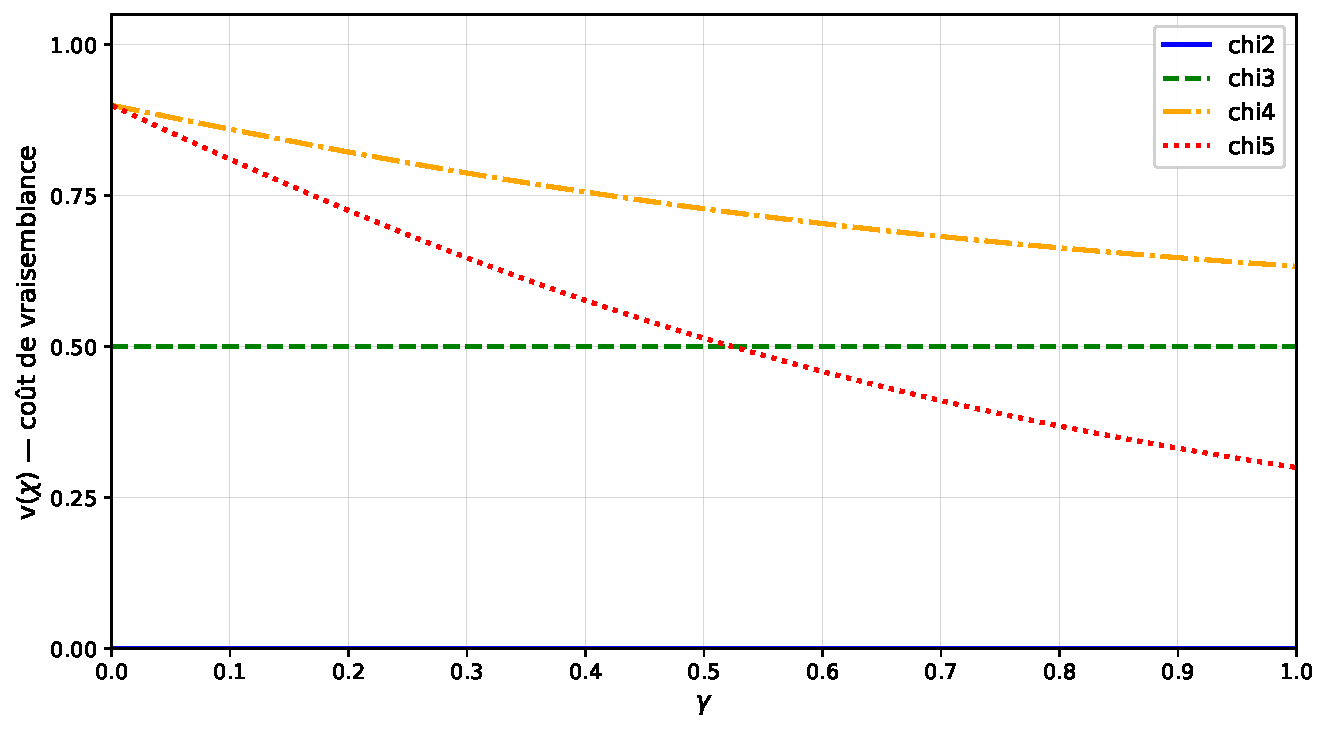
\includegraphics[width=0.6\textwidth]{fig/sensibilite_gamma.pdf}
    \caption{Sensibilité au paramètre $\gamma$ ($agg_\gamma$ early)\\
    Contexte observé : $\chi_1$,  $\lambda_2$ = 1}
    \label{fig:sensi_gamma}
\end{figure}

On observe sur la Figure \ref{fig:sensi_gamma}, l'impact de $\gamma$ sur le coût de vraisemblance. Le contexte causal $\chi_2$ (\textit{VO, boire, Vivant}) contient un unique événement donc sa vraisemblance ne dépend pas de la valeur de $\gamma$. Le contexte causal $\chi_3$ (\textit{V0,vider,VV,}$\emptyset$\textit{,Mort}) ne dépend pas non plus de $\gamma$ alors qu'il contient plus d'un événement. Ce comportement est dû aux scores des événements qui valent tous 0.5 et le fait que l'opérateur respecte une propriété d'idempotence. Lorsque tous les scores à agréger sont égaux, $\gamma$ n'influe pas le résultat. Concernant les contextes causaux $\chi_4$ (\textit{VO, emp, VE,vider,VV,}$\emptyset$\textit{,Mort}) et $\chi_5$ (\textit{VO,emp, VE,anti,VA,boire,Vivant}), ils sont impactés par $\gamma$. Lorsque $\gamma$ est proche de zéro, on ne prend en compte presque uniquement que le premier événement, égal dans les deux scénarios qui est $empoisonner$. Plus la valeur de $\gamma$ augmente, plus on s'intéresse à ce qui se passe en fin de scénario dans $\chi_5$ un antidote est versé, et donc le coût chute plus fortement que dans $\chi_4$. Autour de la valeur $\gamma=0.5$ on observe un chevauchement des courbes de $\chi_3$ et $\chi_5$. Le contexte causal $\chi_5$ devient moins coûteux que $\chi_3$. Cela montre l'importance de fixer correctement $\gamma$. Pour cela, il faut avoir en tête ces valeurs de bascules, même si elles ne sont pas automatiquement présentes, elles peuvent exister. Il est aussi important de fixer $\gamma$ en fonction de la longueur des scénarios que l'on traite. Si les scénarios sont courts favoriser un $\gamma$ relativement faible ($\leq 0.5$) et l'augmenter pour des longueurs plus importantes. 